\section{Multivibrator}
In diesem Versuch soll die Funktionsweise eines Multivibrators  bestimmt werden.
\subsection{Experimentelle Durchf\"urung}
Es wird ein Multivibrator wie in Abbildung 1 dargestellt auf dem Steckbrett aufgebaut. Dabei werden folgende Widerst\"ande verwendet: R$_1$  $=$ 3~$k\Omega$, R$_2$ $=$ 1~$k\Omega$, ein Thermoster von R$_3$ $=$ 6.8~$k\Omega$ bei einer Temperatur von 25$°$~$C$ und eine Kapazit\"at von C$_1$ $=$ 0.1 $\mu F$. Danach wird mit Hilfe eines Oszilloskop die Frequenz bestimmt und mit der erwarteten Frequenz verglichen. Anschlie\ss end wird der Thermistor mit Hilfe eines Eissprays abgek\"uhlt und anhand der neuen Frequenz wird der Temperaturkoeffizient k des Thermistor bestimmt. Es wird angenommen, dass der Thermistor von 25$°$~$C$ auf -40$°$~$C$ abgek\"uht wird.
\begin{figure}[!ht]
\begin{center}
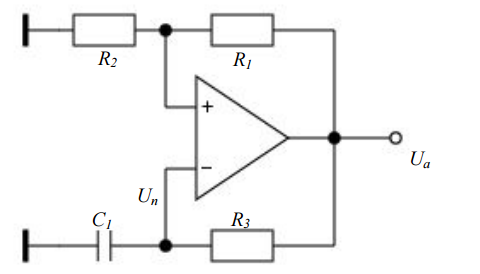
\includegraphics[scale=0.7]{bild/Multivibrator}
\caption{Multivibrator}
\end{center}
\end{figure}
\subsection{Ergebnisse und Diskussion}
Die gemessen Frequenz betrug ca. 670~$Hz$, was um ca. 30\% von der erwarteten Frequenz von 1~$kH$. Die Abweichung l\"asst sich erkl\"aren durch die Temperatur des Thermistorsm die nicht zwangsl\"aufig bei 25$°$~$C$ liegt, sondern tendenziell unter dieser liegt.
\\
Nach abk\"uhlen des Thermistors betrug die Frequenz nur noch 10,41~$Hz$. Mit folgender Formel l\"asst sich damit der neue Widerstandswert des Thermistors bestimmen: 
\begin{equation*}
T = 2\cdot R_3 \cdot C \cdot ln(1+ 2\frac{R_2}{R_1})
\end{equation*}
mit T = $\frac{1}{f}$, f ist die Frequenz. \\
Mit dem neuen berechneten Widerstandswert R$_3$ l\"asst sich $\Delta$R bestimmen.und mit folgender Formel der Temperaturkoeffizient berechnen:
\begin{equation*}
\Delta R = K \cdot \Delta T
\end{equation*}
Unser Ergebnis f\"ur den Temperaturkoeffizient betrug K $=$ 14,36~$\frac{1}{K}$ 
\begin{figure}[!h]
\begin{center}
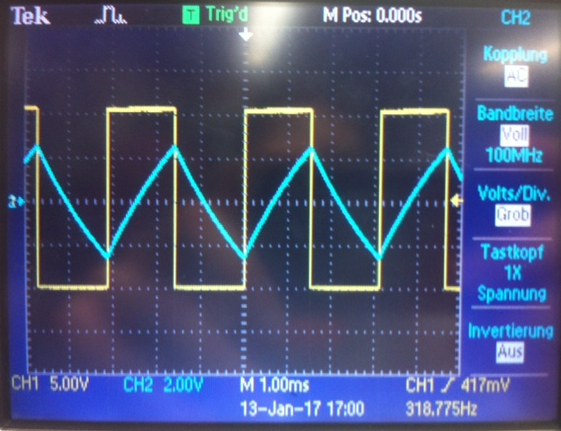
\includegraphics[scale=0.6]{bild/AusgangMulti}
\caption{Ausgangssignal Multivibrator}
\end{center}
\end{figure}
\begin{figure}[!h]
\begin{center}
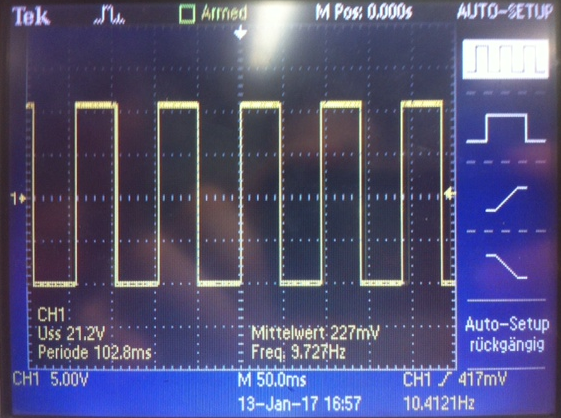
\includegraphics[scale=0.6]{bild/AusgangMultiNachAbkuhlen}
\caption{Ausgangssignal des Multivibrators nach Abk\"uhlen}
\end{center}
\end{figure}
Der Widerstand R$_3$ aus der Schaltung in Abbildung wurde durch eine Diode und einen Widerstand ersetzt, sodass ein Ausgangssignal mit einem Tastgrad ungleich 50\% erzeugt wurde. In Abbildung 4 ist das Ergebnis dieses Vorgangs dargestellt. Man kann erkennen, dass die Periodendauer nicht mehr symmetrisch ist und die Entladezeit des Kondensator schneller ist, dies kann durch die Funktionsweise der Diode erkl\"art werden.
\begin{figure}[!h]
\begin{center}
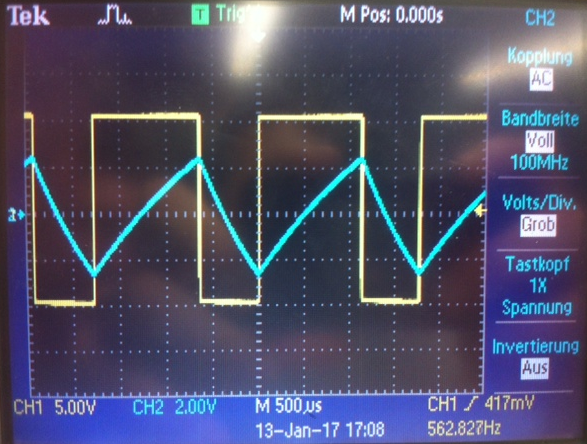
\includegraphics[scale=0.7]{bild/Ausgangauf50}
\caption{Ausgangssignal Multivibrator}
\end{center}
\end{figure}
\newpage